\chapter{Background}
This section aims to provide an overview of the fields of expressive legged robotics relevant to this thessi. Robot design is initially presented along with the state of human-robot interactions. Lastly, we will cover control strategies for legged and expressive motion. 

\section{Physical robot Design}
\textbf{Design choices} \\
Modern robot design choices often take inspiration from biology that leads to robots moving and interacting with the environment in a more natural and efficient manner. Drawing inspiration from the locomotion of running animals and humans, we are able to design robots capable of running, walking, and emoting through natural movement. Leveraging motion beyond pure functionality and efficiency, we may be able to enhance robot-human interaction and collaboration.

\textbf{Legged robotics} \\
During recent years, research and development of legged robotic systems has grown and increased in popularity. Legged robots offer a variety of advantages compared to more traditional wheeled and tracked robots. Legged robots offer superior mobility when faced with uneven or challenging terrain compared to their counterparts. Although legged robots present these advantages, in their current state of development there are numerous challenges as well. Such challenges include high energy consumption, high cost, and low speeds \cite{article}. Despite their many challenges, we see an increase in the use of legged robotics in many industries. Legged robots and their adaptability to challenging terrain and human environments allow for many real-world applications. Examples of such applications include industrial inspection, payload delivery, and search and rescue missions \cite{https://doi.org/10.1002/rob.21839}. 
\newpage
\begin{figure}[H]
    \centering
    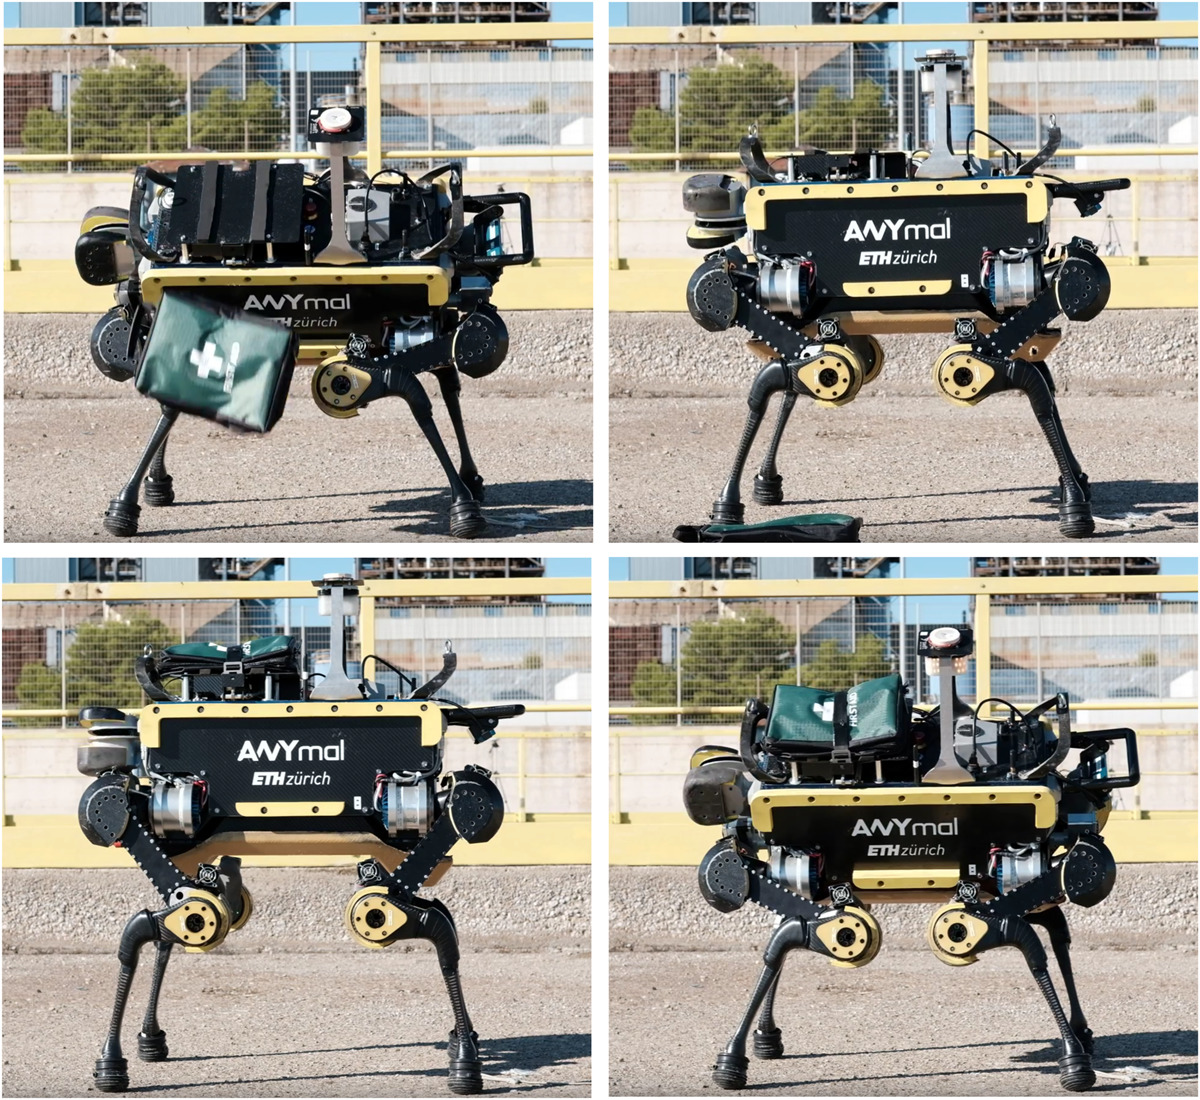
\includegraphics[width=0.8\textwidth]{figures/Payload_delivery.jpg}
    \caption{The ANYmal quadruped robot used in payload delivery applications~\cite{https://doi.org/10.1002/rob.21839}.}
    \label{fig:anymal_payload}
\end{figure}

\section{Legged robot motion control}
\subsection{Biped locomotion design}
\subsection{Inverse/Forward kinematics}
Inverse and Forward Kinematics are mathematical formulas used to calculate the position and configuration of a robot actuator. Forward kinematics is the process of calculating the position and orientation of the end effector based on known joint parameters(angles or displacements). Inverse kinematics is the process of determining the joint parameters needed to achieve a desired position and orientation of the end effector. 

\textbf{Denavit-Hartenberg convention} is a commonly used method for obtaining the forward kinematics model of serial manipulators and simplifying the kinematic analysis. The convention is based on using 4 parameters for each joint to define the relative transformation between coordinate frames attached to adjacent links of a robot manipulator:
\begin{itemize}
  \item \textbf{\( \theta_i \)} -- Joint angle: rotation around the \( z_{i-1} \) axis.
  \item \textbf{\( d_i \)} -- Link offset: translation along the \( z_{i-1} \) axis.
  \item \textbf{\( a_i \)} -- Link length: translation along the \( x_i \) axis (distance between \( z_{i-1} \) and \( z_i \)).
  \item \textbf{\( \alpha_i \)} -- Link twist: rotation around the \( x_i \) axis (angle between \( z_{i-1} \) and \( z_i \)).
\end{itemize}

Each of these parameters defines a physical feature of the robot joint. Three of these parameters will always remain static and the fourth parameter will be dynamic depending on the type of joint. The joints can be simple or more complex. In this case, we focus on hinge joints that rotate around a single axis and prismatic joints that permit linear motion along a single axis. In this thesis, we simply focus on joints with one degree-of-freedom.
To perform the kinematic analysis, we rigidly attach a coordinate frame to each link. In order to represent any arbitrary homogeneous transformation using only four parameters, we must apply 2 constraints:

\begin{itemize}
  \item The axis $x_{i-1}$ is perpendicular to the axis $z_i$
  \item The axis $x_i$ intersects the axis $z_{i-1}$
\end{itemize}

After setting up a system of axes following the constraints, we can calculate the forward kinematics for all joints. With this conversion, each transformation $A_i$ is represented as a product of four basic transformations.

% Requires: \usepackage{amsmath}
\begin{equation}
\begin{aligned}
    A_i &= R_{z,\theta_i} \, \text{Trans}_{z,d_i} \, \text{Trans}_{x,a_i} \, R_{x,\alpha_i} \\
    &= \begin{bmatrix}
        \cos \theta_i & -\sin \theta_i & 0 & 0 \\
        \sin \theta_i & \cos \theta_i & 0 & 0 \\
        0 & 0 & 1 & 0 \\
        0 & 0 & 0 & 1 \\
    \end{bmatrix}
    \begin{bmatrix}
        1 & 0 & 0 & 0 \\
        0 & 1 & 0 & 0 \\
        0 & 0 & 1 & d_i \\
        0 & 0 & 0 & 1 \\
    \end{bmatrix}
    \begin{bmatrix}
        1 & 0 & 0 & a_i \\
        0 & 1 & 0 & 0 \\
        0 & 0 & 1 & 0 \\
        0 & 0 & 0 & 1 \\
    \end{bmatrix}
    \begin{bmatrix}
        1 & 0 & 0 & 0 \\
        0 & \cos \alpha_i & -\sin \alpha_i & 0 \\
        0 & \sin \alpha_i & \cos \alpha_i & 0 \\
        0 & 0 & 0 & 1 \\
    \end{bmatrix}
    \\
    &= \begin{bmatrix}
        \cos \theta_i & -\sin \theta_i\cos \alpha_i & \sin \theta_i\sin \alpha_i & a_i\cos \theta_i \\
        \sin \theta_i & \cos \theta_i\cos \alpha_i & -\cos \theta_i\sin \alpha_i & a_i\sin \theta_i \\
        0 & \sin \alpha_i & \cos \alpha_i & d_i \\
        0 & 0 & 0 & 1 \\
    \end{bmatrix}
\end{aligned}
\end{equation}
From here we can form the overall transformation matrix as a product of the homogeneous transformation matrices:
\begin{equation}
   T_n^0 = A_1 A_2 \cdots A_n
\label{placeholder}
\end{equation}


\section{Expressive Robot motion control}
The relationship between robot movement and our perception has been an exciting and recognized area of research \cite{van_den_brule_robot_2014}. Robots are highly capable and are used in a wide variety of situations. When placed in environments where they interact with humans, they have an innate ability to communicate with their human counterparts. Even when disregarding verbal communication, robots are able to communicate through movement and use their embodiment to generate expressive movements in addition to completing tasks. Using expressive and communicative movements, robots can provide additional information to their human partners.

The general approach to motion control is done through developing trajectories and controllers that produce fast, accurate, and smooth motion while maintaining high repeatability in controlled environments. This is typically done through feedback control loops that allow the robot to react to its environment.  This approach to control is most commonly applied in industrial settings where robot manipulators operate with a fixed or mobile base operating in isolation from humans. The resulting motion will be rather machine-like, as it moves with consistent motion in straight lines. We have also seen that motion control for legged robotic systems has been an active area of research\cite{wieber_modeling_2016}. When working with legged systems, the focus of developing trajectories and control becomes more challenging as we also have to maintain balance, which is especially challenging in biped robots.

Robots are now being used outside isolated industrial settings and are increasingly expected to interact with humans in contexts like interactive art, companionship, collaboration, and assistance. These new applications introduce new challenges in motion generation as the performance can no longer be evaluated by objective criteria like precision and speed, but rather by the perception of the user.

\subsection{Animating robots}
When developing algorithms for expressive motions, there are multiple areas of research from which to draw inspiration. The field of character animation has mastered the art of endowing digital characters with the illusion of life. Bringing this level of lifelike expression to robots has been an aspiration for some time. An approach proposed by Van Breemen in \cite{breemen_bringing_2004} suggests applying the principles of character animation to bring robots to life. Breemen also presented an animation engine that combines multiple interactive robot behaviors with believable robot animations\cite{van_breemen_animation_2004}. Takayama et al. built further on this idea in \cite{takayama_expressing_2011} and found that drawing from animation principles allowed the robot to illustrate forethought and reaction. This was also found to make people more sure of their interpretations of the robot's behavior while also making the robot appear more appealing, approachable, capable, and intelligent even when failing functional tasks at hand. 

In the work of Thomas and Johnson \cite{thomas_disney_1981}, they documented how Walt Disney Studios practices their methods of animation until they derived a series of methods that produced predictable results. These methods were then deemed the fundamental principles of animation. These principles are not verified by science but are widely used in a variety of animated media. The principles are as follows: 
\begin{itemize}
    \item \textbf{Squash and Stretch:} Characters and objects should squash and stretch with their action, although they do not completely lose their shape. 
    \item \textbf{Anticipation:} Major action should be telegraphed such as reaching back before throwing an object. 
    \item \textbf{Staging:} An action should be clear to the audience. For example, the audience should understand the action by only viewing it in silhouette.
    \item \textbf{Straight Ahead Action and Pose to Pose:} This principle describes how to draw an action. Drawing straight ahead involves starting to draw and simple continuing until the action is completed. Pose to pose implies that specific poses are desired in an action and are choreographed before the actual animation.
    \item \textbf{Slow In and Slow Out:} The speed of a motion is not the same during the time that it is performed. Action is slower at the beginning and end. 
    \item \textbf{Arcs:} Move limbs in arcs as opposed to of straight up-down and left-right motions. 
    \item \textbf{Secondary Action:} Create complementary actions that emphasize the main action. For example, a character puts on a coat while walking out the door. 
    \item \textbf{Timing:} Changes in number of frames that are between a start and stop determines the speed of the action, thereby increasing the number of frames and decreasing the speed of the action. 
    \item \textbf{Exaggeration:} Exaggerated action ensures that it is easier to understand the feelings of a character. 
    \item \textbf{Solid Drawing:} Drawings should look plausible and three-dimensional and twinssymmetrical limbs on a character—should be avoided, since it makes characters look stiff.
    \item \textbf{Appeal:} All the characters should be appealing whether one is expected to sympathize with them or despise them. 
\end{itemize}

These principles can also be employed by physical systems in order to make systems appear more lifelike. While the field offers a wide range of techniques, this section focuses on a subset that is particularly relevant to the goals of this project.

Commonly applied principles include \textit{Secondary action} and are applied in \cite{park_generation_2015} to help provide increased readability and credibility of behaviors and expressions of robots. Similar principles are applied in the work of Asselborn et al. \cite{asselborn_keep_2017} they explored the effects of a robot's subconscious gestures made during moments when idle on the perception of children. In the conclusion of this work, a clear correlation was found between the adaptor movements and the humanity and friendliness perception. 

Other principles being used in robot motion include \textit{pose to pose} where a series of key poses are defined first, and the movement between them is generated at a later stage. In Beck et al. \cite{beck_emotional_2012} emotional expressions were constructed by extracting key poses from actor performances, which were then implemented on the Nao robot. Each pose was associated with a specific emotional state validated through user studies. By blending key poses, the robot was enabled to convincingly display emotions through expressive body language.

Other animation principles used to enhance the expressive capabilities of robots include \textit{Exaggeration} and is used to make it easier to interpret what the robot is doing. Exaggeration is utilized with secondary action in \cite{park_generation_2015} in way to make it easier for participants to understand the emotions displayed by the robot.

 
\subsection{Reinforcement learning}
While animation principles can guide the design of expressive robot behaviors, reinforcement learning offers a data-driven framework to generate expressive motion autonomously. Many take advantage of RL when generating expressive motion for robots rather than relying on pre-programmed movements and animations. In the work of Grandia et al. \cite{grandia_design_2024}, reinforcement learning is used to generate expressive motion by training control policies to imitate animations designed by artists. By using a policy gradient approach, the robot character learns perpetual, periodic, and episodic motions based on high-level control commands while still maintaining balance. The reward function is designed to reward accurate movement and survival, enabling the robot to robustly perform expressive motion.